\section{Messaufbau}


\begin{figure}[H]
    \centering
    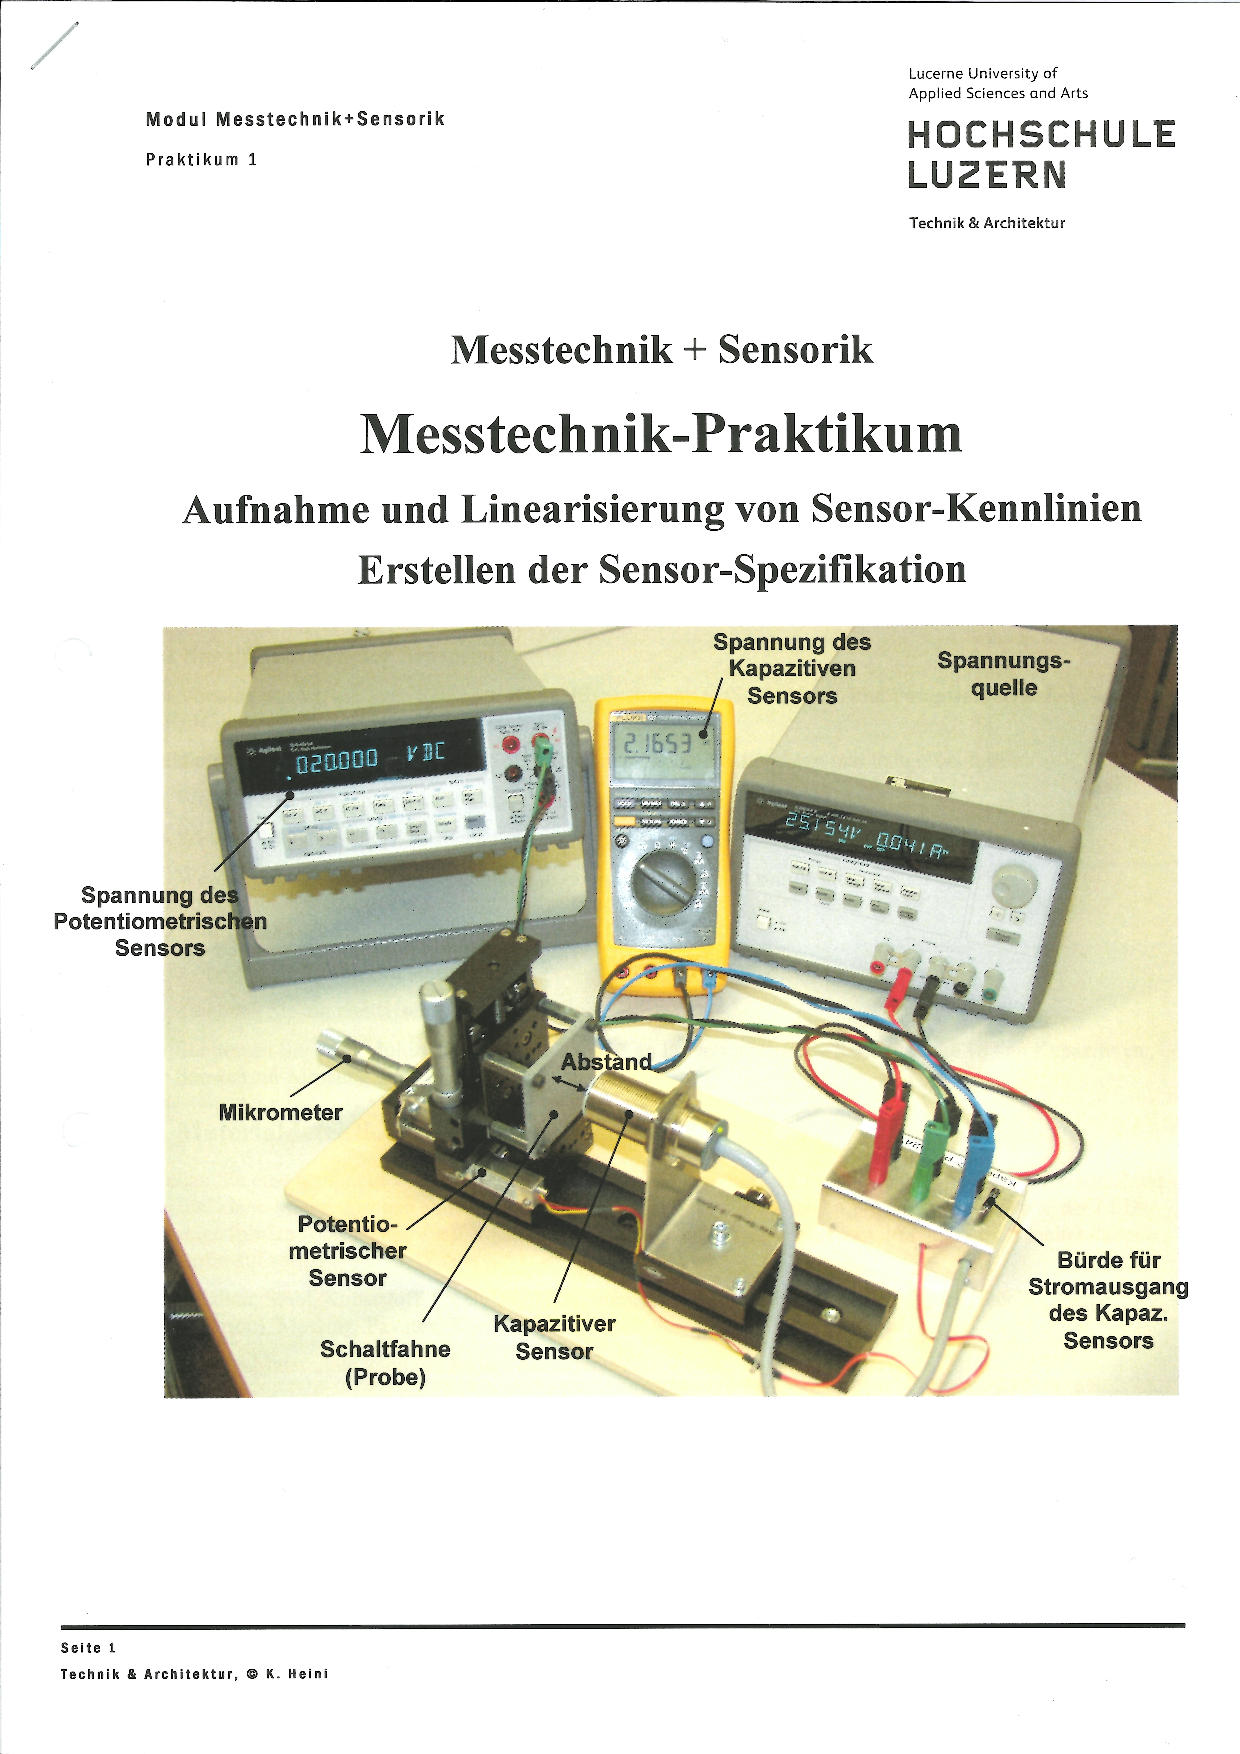
\includegraphics[scale=0.8,trim={0.5cm 6cm 0 10.5cm},clip]{pic/aufbau.pdf}
    \caption{Messaufbau}
    \label{fig:messaufbau}
\end{figure}

Folgende Messgeräte wurden verwendet: \\

\begin{tabular}{ l | l | l}
    \hline
    Hersteller & Typ                 & Verwendung                  \\ \hline
    Agilent    & E3634A Power Supply & Speisung Spannungsteiler    \\ \hline
    Agilent    & 34401A Mulitmeter   & Spannung Potentiometer      \\ \hline
    Fluke      & 187 TRMS multimeter & Spannung kapazitiver Sensor \\ \hline
    Rechner    & KAS-80-A14-IL       & kapazitiver Sensor          \\ \hline
    Genge\& Thoma & HP15C               & Potentiometrischer Sensor   \\ \hline
\end{tabular}


\subsection{Elektrisches Ersatzschaltbild}


Ist das Messgerät genug hoch-$\Omega$ oder wird der Spannungsteiler belastet?






\clearpage